\section{An infinite-product representation}
\label{a:sec:product}

Take the nonlinear map for the survival probability,
\begin{equation*}
S_{n+1} = 2pS_n - pS_n^2,\qquad S_0=1,
\end{equation*}
and substitute $S_n = 2w_n$. This gives
\begin{equation}
\label{a:eq:logistic}
w_{n+1} = 2p\,w_n(1-w_n) = r\,w_n(1-w_n),
\qquad r = 2p,\quad w_0 = \tfrac12 ,
\end{equation}
which is the logistic map --- the same map that exhibits the period-doubling route
to chaos as $r$ increases from $0$ to $4$ (\cref{a:fig:period_double}). The
subcritical window is $r\in[0,1)$, at the extreme left of that picture, where the
origin is a globally attracting fixed point. That this innocuous corner of the
logistic family is nevertheless enough to obstruct a closed form is the substance
of \cref{a:sec:ht}.

\begin{figure}[ht]
    \centering
    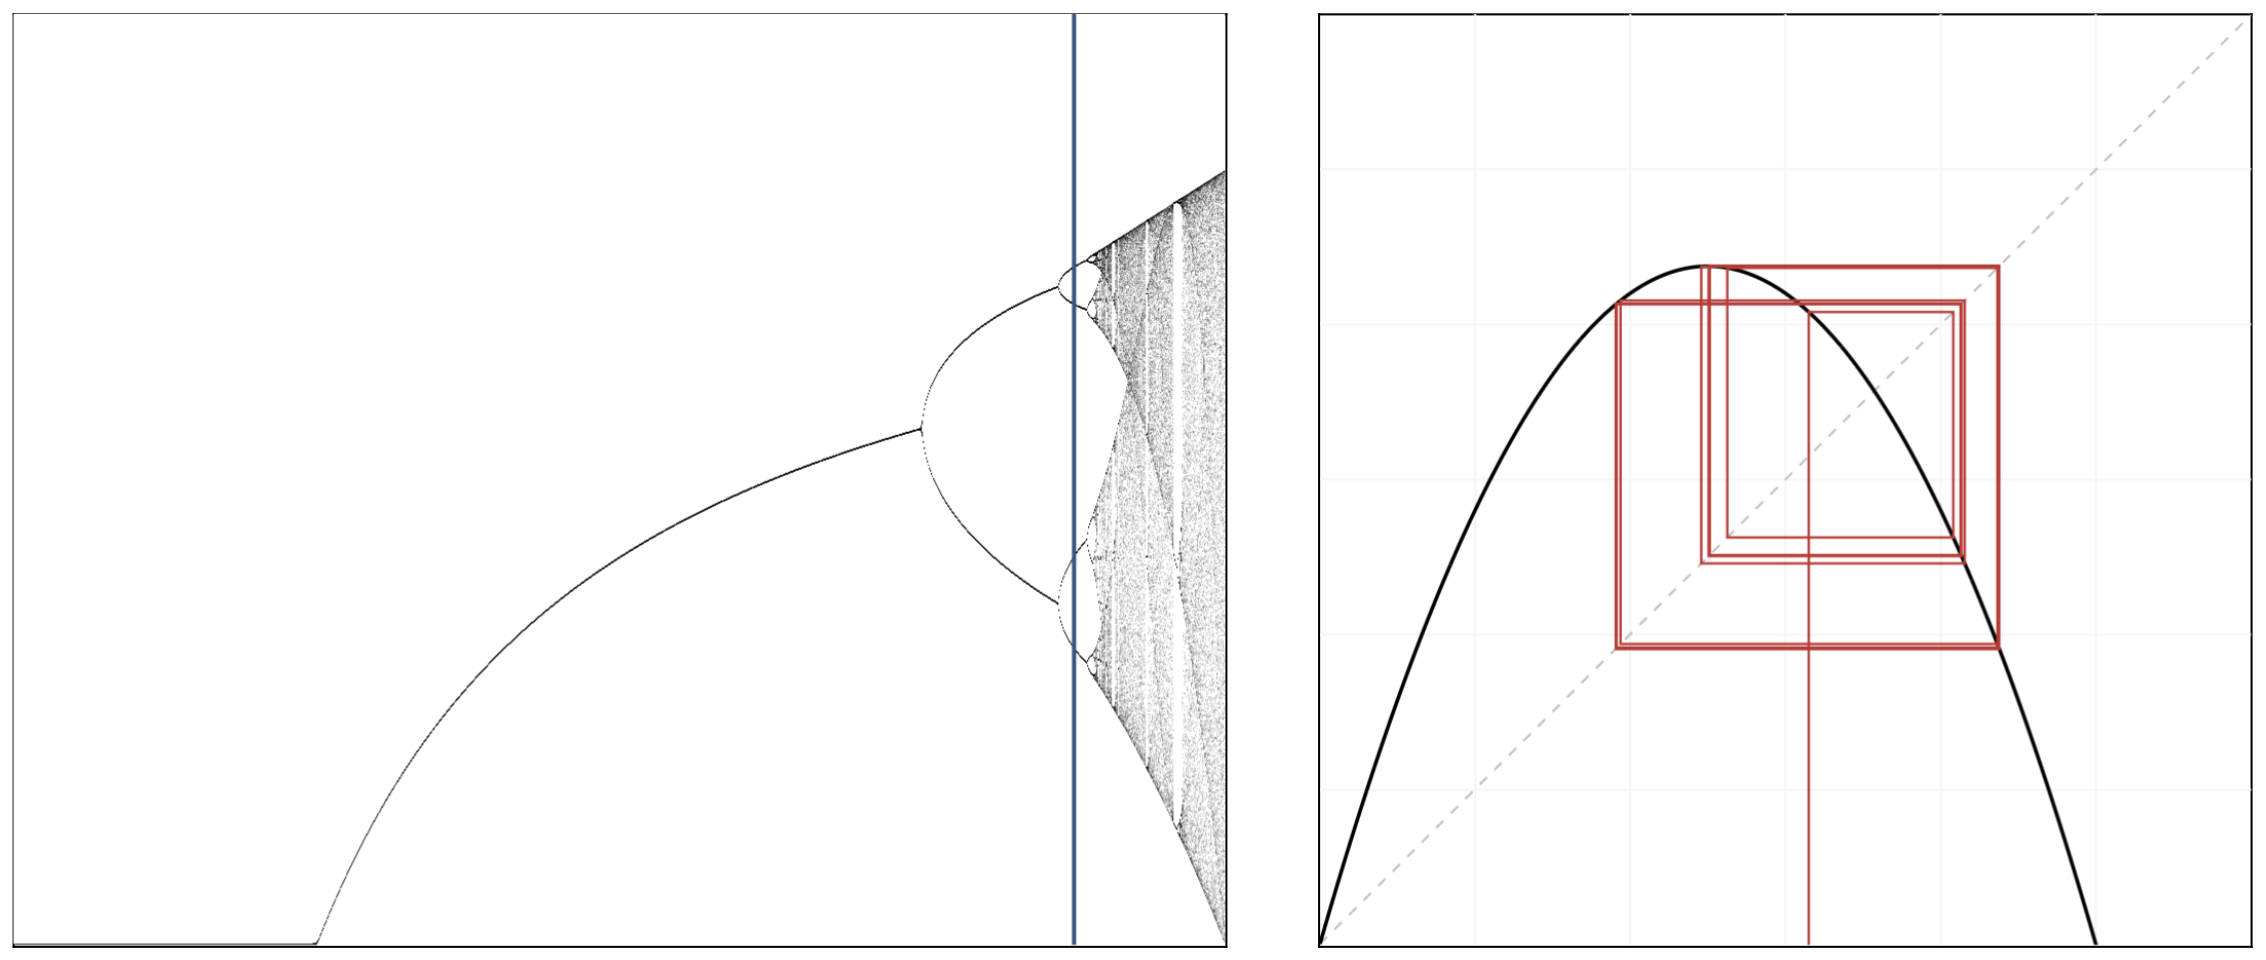
\includegraphics[width=0.86\textwidth]{figures/period_double.png}
    \caption{Bifurcation diagram of the logistic map $w\mapsto rw(1-w)$, showing
    the period doubling of stable states and the onset of chaos. The blue sample
    line on the left is at $r=3.5255$; the right-hand plot shows a trajectory of
    the map at the same $r$. The regime relevant to subcritical branching is
    $r=2p\in[0,1)$, off the left-hand edge of this diagram, where the dynamics are
    as simple as they can be.}
    \label{a:fig:period_double}
\end{figure}

In terms of $w$, \cref{a:eq:Apdef} reads
\begin{equation}
\label{a:eq:Aw}
A(p) = \lim_{n\to\infty}\frac{S_n}{(2p)^n} = 2\lim_{n\to\infty}\frac{w_n}{r^n} .
\end{equation}
Any sequence can be written as a telescoping product,
\begin{equation*}
x_n = x_0\lrb{\frac{x_1}{x_0}}\lrb{\frac{x_2}{x_1}}\cdots\lrb{\frac{x_n}{x_{n-1}}}
= x_0\prod_{k=0}^{n-1}\frac{x_{k+1}}{x_k},
\qquad\text{so}\qquad
\lim_{n\to\infty}x_n = x_0\prod_{k=0}^{\infty}\frac{x_{k+1}}{x_k},
\end{equation*}
and applying this with $x_n = w_n/r^n$ the ratio simplifies at once:
\begin{equation*}
\frac{x_{k+1}}{x_k}
= \frac{w_{k+1}}{w_k}\cdot\frac1r
= \frac{rw_k(1-w_k)}{w_k}\cdot\frac1r
= 1-w_k .
\end{equation*}
Hence, with $x_0 = w_0 = \tfrac12$ and $A(p) = 2\lim_n x_n$,
\begin{equation*}
A(p) = 2\cdot\tfrac12\prod_{k=0}^{\infty}(1-w_k) = \prod_{k=0}^{\infty}(1-w_k),
\end{equation*}
and pulling out the factor $1-w_0=\tfrac12$,
\begin{equation}
\label{a:eq:prodFormula}
A(p) = \frac12\prod_{k=1}^{\infty}(1-w_k)
= \frac12\prod_{k=1}^{\infty}\lrb{1-\frac{S_k}{2}} .
\end{equation}

\subsection{Convergence, and existence of the limit}
\label{a:sec:prodconvergence}

For $0<w_k<1$ the infinite product $\prod_{k\ge1}(1-w_k)$ converges to a strictly
positive limit if and only if $\sum_{k\ge1}w_k<\infty$. From \cref{a:eq:logistic}
with $0<r<1$ and $0<w_n<1$ we have $w_{n+1}<rw_n$, so by induction
$w_n\le w_0r^n$; since $0<r<1$ this bound is summable, and the product converges
to a positive finite value. That also establishes what was asserted in
\cref{a:sec:setupAp}: the limit \cref{a:eq:Apdef} defining $A(p)$ exists and lies
strictly between $0$ and $\tfrac12$ for $p\in(0,\tfrac12)$.

The finite partial products
\begin{equation}
\label{a:eq:partialproduct}
A_N(p) = \frac12\prod_{k=1}^{N}\lrb{1-\frac{S_k}{2}}
\end{equation}
decrease monotonically to $A(p)$, so every truncation is a rigorous upper bound. A
useful lower bound accompanies it: since $\prod_k(1-a_k)\ge1-\sum_ka_k$ for
$a_k\in[0,1]$, and since $w_{k+1}\le rw_k$ gives
$\sum_{k>N}w_k\le w_{N+1}/(1-r)$,
\begin{equation}
\label{a:eq:tailbound}
A_N(p)\lrb{1-\frac{w_{N+1}}{1-r}} \;\le\; A(p) \;\le\; A_N(p)
\end{equation}
whenever the left factor is positive. The bracket provides a certified stopping
criterion for numerical evaluation: it is stronger than merely observing that
successive iterates have stopped changing, and it is what \cref{a:sec:practical}
uses to decide when enough factors have been taken.

\subsection{Is this an advance?}
\label{a:sec:advance}

Only a modest one. \Cref{a:eq:prodFormula} is exact and its partial products
decrease monotonically, so truncating gives a rigorous upper bound on $A(p)$ at
every order, which the raw ratio $S_n/(2p)^n$ does not. But computing the factors
still requires iterating the nonlinear map to generate the $S_k$, so the
near-critical difficulty is untouched: as $p\to\tfrac12^-$ the number of factors
needed grows without bound. What the product does supply is a route to the sharper
result of the next section.
